\section{Конструкторская часть}

В данном разделе разработан метод программной реализации доверенной среды исполнения с помощью виртуализации процессоров архитектуры ARM: изложены особенности метода, представлена его формализация в виде диаграмм IDEF0 и схем алгоритмов.

\subsection{Особенности метода}

Доверенная среда исполнения в общем смысле -- это изоляция ресурсов (памяти и периферии) от основной ОС, которая считается недоверенной. Такой тип изоляции, на платформах ARM, можно достичь с помощью механизма ARM Virtualzation. 

Как уже было сказано ранее, в ARM код операционных систем выполняется на уровне привилегий EL1. Механизм визуализации добавляет в архитектуру ARM ещё два режима исполнения кода на уровне EL1: гостевой (guest) и хостовый (host). Таким образом, в системе может одновременно присутствовать и гостевая операционная система и хостовая.

В режим host операционная система имеет прямой доступ к аппаратным ресурсам, в отличии от режима guest, в котором доступ к ресурсам ограничен. Таким образом, гостевая операционная система изолируется от хостовой.

На рисунке \ref{fig:arm-virtualization} представлена схема режима работы процессоров архитектуры ARM с поддержкой ARM Virtualzation.

\begin{figure}[h]
	\centering
	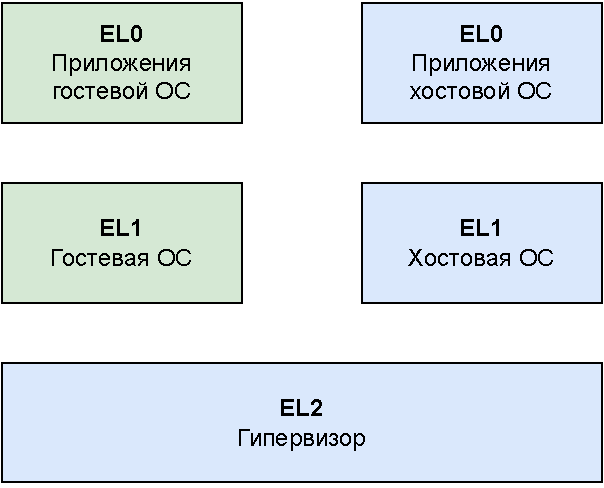
\includegraphics[width=\textwidth]{img/arm-virtualzation.pdf}
	\caption{Режимы работы процессоров ARM с аппаратной поддержкой виртуализации}
	\label{fig:arm-virtualization}
\end{figure}

Шаги метода программной реализации доверенной среды исполнения с помощью виртуализации процессоров архитектуры ARM можно описать следующим образом:

\begin{enumerate}
	\item в момент передачи управления ARM TrustZone, все ядра процессора необходимо перевести в режим работы гипервизора;
	\item хостовую ОС нужно перевести в режим исполнения guest mode;
	\item передать гипервизору для общения с периферией заранее зарезервированную память, которой владеет ARM TrustZone.
	\item после того, как ARM TrustZone выполнила свою работу, выйти из режима гипервизора и передать зарезевированную память обратно;
	\item хостовую ОС перевести в режим исполнения host mode.
\end{enumerate}

Гостевая операционная система не может получить доступ к памяти, которой владеет гипервизор. В хостовом режиме исполнения, она так же не может получить к ней доступ, потому что ей управляет ARM TrustZone. Таким образом, обеспечивается изоляция ресурсов от недоверенной ОС.

\subsection{Формальное описание метода}

На рисунке \ref{fig:idef0-0} представлена IDEF0 диаграмма разрабатываемого метода.

\begin{figure}[h]
	\centering
	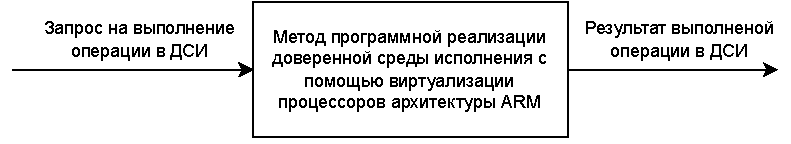
\includegraphics[width=\textwidth]{img/idef0-0.pdf}
	\caption{IDEF0 диаграмма разрабатываемого метода}
	\label{fig:idef0-0}
\end{figure}

На рисунке \ref{fig:idef0-1} представлена детализированная IDEF0 диаграмма разрабатываемого метода.

\begin{figure}[h]
	\centering
	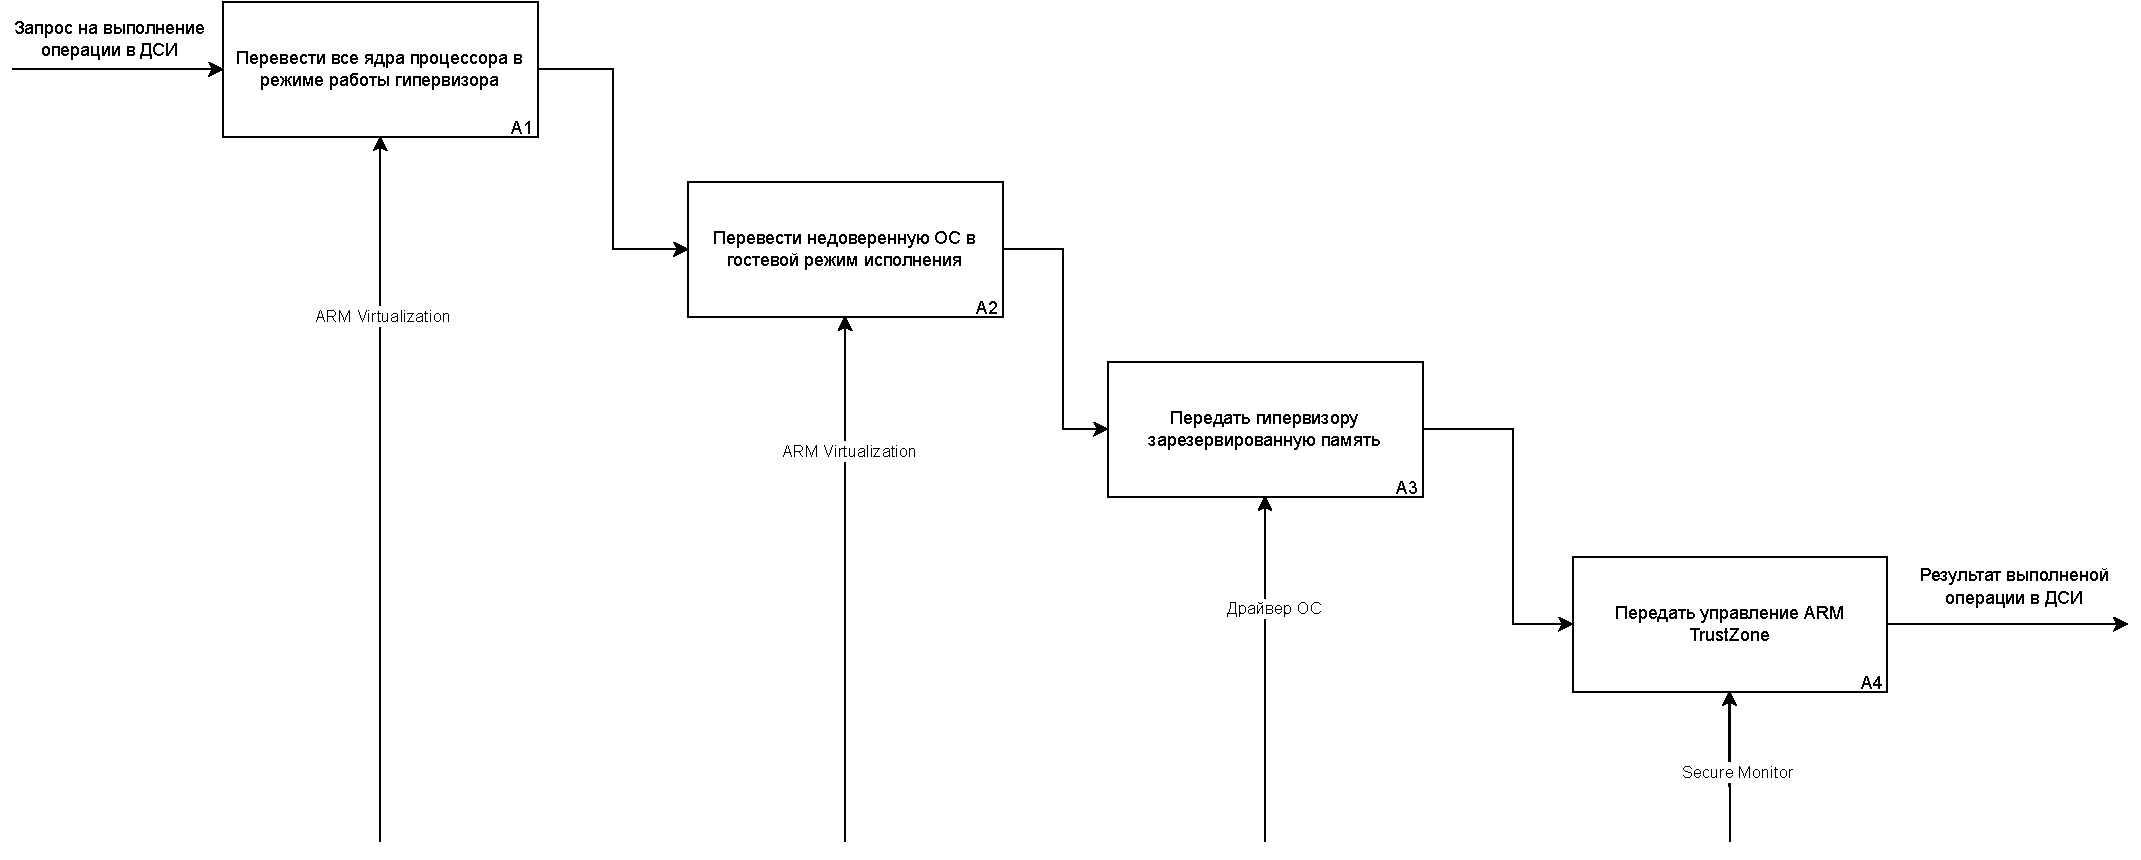
\includegraphics[width=\textwidth]{img/idef0-1.pdf}
	\caption{Детализированная IDEF0 диаграмма разрабатываемого метода}
	\label{fig:idef0-1}
\end{figure}

\subsection{Описание используемых алгоритмов}

\subsubsection{Алгоритм перехода в режим исполнения гипервизора}

На рисунке \ref{fig:algo-1} представлена схема алгоритма перехода в режим исполнения гипервизора. Входными данными этого алгоритма является система, которая уже выполняется с уровнем привилегий EL1.

\begin{figure}[h]
	\centering
	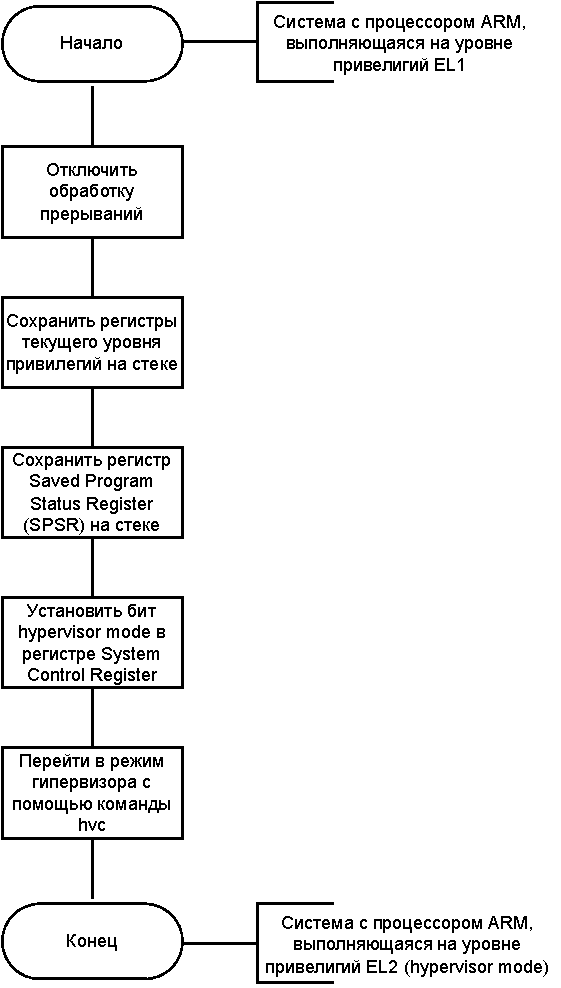
\includegraphics[scale=1.3]{img/algo1.pdf}
	\caption{Алгоритм перехода в режим исполнения гипервизора}
	\label{fig:algo-1}
\end{figure}

\pagebreak
